% siminos/reversal/Hill.tex      pdflatex LC21; bibtex LC21
% temporary: siminos/spatiotemp/chapter/LC21Hill.tex
% $Author: predrag $ $Date: 2021-12-24 01:25:20 -0500 (Fri, 24 Dec 2021) $

%\renewcommand{\Ssym}[1]{{\ensuremath{m_{#1}}}}
\renewcommand{\statesp}{state space}
\renewcommand{\Statesp}{State space}
\renewcommand{\stateDsp}{state-space}
\renewcommand{\StateDsp}{State-space}

\section{% Hill's formula:
         Stability of an orbit vs. its time-evolution stability}
\label{s:LC21Hill}
% PC started with: siminos/kittens/Hill.tex  2021-08-19

In 1878-1886 a study of stability of the planar motion of the moon around
the earth led  Hill to the \emph{Hill's formula}\rf{Hill86}
\beq
\left|\Det\jMorb_c \right|= \left|\det (\id - \jMat_c)\right|
%\,.
\ee{detDet}
which relates the characteristic polynomial of the for\-ward-in-time
evolution {\po} Floquet stability matrix (monodromy matrix) $\jMat_p$ to the
determinant of the global {\jacobianOrb} $\jMorb_p$ (in Lagrangian settings,
the Hessian, the second variation of the action functional).
The discrete-time Lagrangian systems' Hill's formula
% \refeq{MacMei83(17)}
that we use here was derived by Mackay and Meiss\rf{MacMei83} in 1983.

Hill was lucky: he computed $\Det\jMorb_c$ in a $3\times 3$ Fourier modes
matrix approximation, which turned out to be quite a good approximation.
But this is a remarkable formula, especially in the limit of
$\cl{}\to\infty$ infinitesimal time steps, that relates a
field-theoretic, $\infty$\dmn\ \emph{functional} {\HillDet}
$\Det\jMorb_c$ to a determinant of the finite, $[d\times{d}]$ matrix
$\jMat_c$, and it took \Poincare\rf{Poinc1886} to prove that Hill's
Fourier modes calculation is correct in the continuum limit.

the {\jacobianOrb}  and the temporal evolution
\refeq{PV2config} stability ${{\hat{\mathbf{\jMat}}_{p}}}$ are related by
the remarkable (discrete time) Hill's formula\rf{MacMei83,BolTre10}
which expresses the  {\HillDet} of the arbitrarily large \jacobianOrb\
$\jMorb$  in terms of a determinant of a small
[$2\speriod{}\!\times\!2\speriod{}$] time-evolution \jacobianM\
$\hat{\mathbf{\jMat}}_p$.


While first discovered in a Lagrangian setting, Hill's formulas are much
more general, with the Lagrangian formalism of
\refrefs{MacMei83,TreZub09,BolTre10,kooknewt} --just a special case-- only
getting in way of understanding them.
As the formula is fundamental to the formulation
of the \spt\ chaotic field theory, we shall
rederive it here in several ways, relying on nothing more than elementary
linear algebra, in order to emphasize that formula applies to dissipative dynamical
systems as well, from the Bernoulli map to \NS\ and
\KS\rf{GudorfThesis,GuBuCv17}.


\bigskip

Assume that a \po\ $\ssp(\period{p}+\zeit)=\ssp(\zeit)$ of a continuous
time flow
\(
\dot{\ssp}=\vel(\ssp)
\)
is known `numerically exactly', that is to say, to arbitrary (but not
infinite) precision. One way to present the solution is to give a single
point $\ssp(0)$ in the orbit, and let the reader reconstruct the orbit
$p$ by integrating forward in time,
$\ssp(\zeit)=\hat{\map}^\zeit(\ssp(0))$, $\zeit\in[0,\period{p}]$.

However, for a linearly unstable \po\ a single point does not suffice to
present the orbit, because there is always a finite `Lyapunov time'
$\zeit_{Lyap}$  beyond which $\hat{\map}^\zeit(\ssp(0))$ has lost all memory of
the \po\ $p$. This problem is particularly severe in searches for {`\ecs
s'} embedded in turbulence, where even the shortest period solutions have
to be computed to the (for everyday fluid dynamics excessive) machine
precision\rf{GHCW07,channelflow,openpipeflow} in order to complete the
first return to the initial state.

Instead of relaying on for\-ward-in-time numerical integration,
\emph{global methods} for finding periodic orbits\rf{ChoGuck99} view them
as equations for the vector fields $\dot{\ssp}$ on spaces of closed
curves. In numerical implementations one discretizes the \po\  $p$ into
sufficiently many short
segments\rf{auto,GM00aut,ChoGuck99,DingCvit14,DCTSCD14}, and lists a
point for each segment
\beq
p=(\ssp_1,\ssp_2,\cdots,\ssp_\cl{p})
\,.
\ee{nXdCycle}
For a $k$\dmn\ discrete time map $\hat{\map}$ obtained by cutting the flow by a
set of {\PoincSec s}, with the \po\ $p$ of discrete period $\cl{p}$,
every segment can be reconstructed by a short time integration, and
satisfies
\beq
\ssp_{k+1}=\hat{\map}(\ssp_k)
\,,
\ee{CyclePntErr}
to high accuracy, as for sufficiently short times the exponential
instabilities are numerically controllable.


\bigskip

The temporal Bernoulli {\jacobianOrb} %\refeq{1stepVecEq},
$\jMorb=\partial/\partial\zeit-(s-1)\,\shift^{-1}$ is a differential
operator whose determinant one usually computes by a Fourier transform
diagonalization (see \refsect{sect:LC21recip1d}). The Fourier discretization
approach goes all the way back to Hill's 1886 paper\rf{Hill86};


\bigskip

In preparing this summary we have found expositions of Lagrangian
dynamics for discrete time systems by MacKay, Meiss and
Percival\rf{MKMP84,meiss92}, and Li and Tomsovic\rf{LiTom17b} particulary
helpful.

This formula was derived by Mackay and Meiss\rf{MacMei83} and
Allroth\rf{Allroth83} (Allroth eq.~(12)). It applies to general
``one-degree-of-freedom'' systems, \ie, 1D lattices with only the nearest
neighbor interactions. For a finite set of neighbors, \ie, higher\dmn\
discrete-time systems, Allroth\rf{Allroth83} has some partial results in the
context of Frenkel-Kontorova models.

{\HillDet}\rf{MacMei83,BolTre10,Verdiere07};
discrete Hill's formula and the Hill discriminant, Toda lattice\rf{Toda89}.

Toda\rf{Toda89} % {\em Theory of Nonlinear Lattices},
Chapt.~4.{\em Periodic Systems}

Toda studies the classical mechanics of one-dimensional
lattices (chains) of particles with nearest neighbor interaction; they
are discrete and infinite in space, continuous in time.

The {\em inverse scattering method} for an infinite lattice makes use of
the discrete Schrodinger equation. For periodic systems this gives a
discrete Hill's equation, and in place of the scattering data, it is
convenient to use the spectrum of the discrete Hill's equation.
 Thus the initial value problem reduces to the inverse problem
(Jacobi's inverse problem), or inverse spectral theory.

Toda discrete Hill's equation is continuous in time, so presumably the most
of the work is for stationary states.

He works with a 3-term recurrence (4.1.3a), and defines a 2-configuration
monodromy matrix (4.1.11).

For special values of A, the solution of (4.1.4) can be periodic, but
more generally it is relative periodic (4.1.16), or the Bloch function
(it's existence given by the Floquet theorem).
His \jacobianOrb\ (4.1.28) has variable diagonal and off
diagonal elements, corresponding to nontrivial nonlinear solutions for
$d=1$ lattice.

Historically,  in \po\ theory
calculations one always computes $\jMat_\Mm$. However, as we shall show
here, and in more generality in \refsect{s:Hill}, it is the {\HillDet}
$\Det\jMorb$ that is the computationally robust quantity that one should
evaluate.

\begin{quote}
A succinct  explanation of the Hill's formula:\\
If you evaluate stability of the 3-term recurrence \refeq{JiKoKr20(2)} on
a periodic lattice you get the {\jacobianOrb} $\jMorb$;
if you evaluate it by multiplying the `two-configuration representation'
matrix $\jMps$, you get the `time evolution' side of the Hill's formula.
\end{quote}


% PC 2021-10-23
%     moved from siminos/spatiotemp/chapter/LC21Bernoulli.tex
\subsection{{\HillDet} for a $d$-component lattice field}
\label{s:LC21notHill}   % was {exam:Hill1stOrd}
% maybe call this {Hill's formula for a general first-order system}
% siminos/spatiotemp/Examples/examHill1stOrd.tex

The {\jacobianOrb} $\jMorb_{\zeit\zeit'}$ \refeq{jacobianOrb} is a
high-\dmn\ linear stability matrix for the extremum condition
$F[\Xx_c]=0$, evaluated on the {\lattstate} $\Xx_c$. How is the stability
so computed related to the conventional dynamical systems'
for\-ward-in-time stability? To motivate the answer in its generality,
consider a temporal lattice with a set of $d$ fields
$\ssp_{\zeit}=\{\ssp_{\zeit,1},\ssp_{\zeit,2},\dots,\ssp_{\zeit,d}\}$ on
each lattice site $\zeit$, and time evolution given by a $d$\dmn\ map
$\ssp_{\zeit+1}=\hat{\map}(\ssp_{\zeit})$.
A period-$\cl{}$ {\lattstate} \refeq{pathBern} thus
satisfies site-by-site the first-order difference equation
\beq
\ssp_{\zeit} - \hat{\map}(\ssp_{\zeit-1}) = 0
    \,,\qquad
\zeit=1,2,\cdots,\cl{}
\,.
\ee{1stepNonlimTemp}
A small deviation $\Delta\Xx$ from $\Xx_p$ then satisfies the linearized condition
\beq
\Delta\ssp_{\zeit} - \shift^{-1}\jMat_{\zeit}\,\Delta\ssp_{\zeit} = 0
\,,\qquad
(\jMat_{\zeit})_{ij}
=
        %\left.
        \frac{\partial \flow{}{\ssp_\zeit}_i }
             {\partial \ssp_j                }
        %\right|_{\ssp_{j}=\ssp_{\zeit,j}}
\,,
\ee{d-1stepJac2}
where $\jMat_{\zeit}$ is the 1-time step $[d\!\times\!{d}]$
\jacobianM, evaluated on lattice site $\zeit$.

It suffices to work out a temporal period $\cl{}=3$ example to understand
the calculation for any period. In terms of the $[3d\!\times\!3d]$
generalized \refeq{hopMatrix} block shift matrix $\shift$, the \jacobianOrb\
\refeq{jacobianOrb} has block matrix form
\beq
\jMorb_p \,=\,
\id-\shift^{-1}\jMat
\,,\quad
\shift =
\left[
\begin{array}{ccc}
0     & \id_d& 0   \\
0     & 0     & \id_d\\
\id_d& 0     & 0
\end{array}
\right]
\,,\quad
\jMat =
\left[
\begin{array}{ccc}
\jMat_1 & 0 & 0 \\
0 & \jMat_2 & 0  \\
0 & 0 & \jMat_3
\end{array}
\right]
\,,
\ee{3shift}
where $\id  $ is the $d$\dmn\ identity matrix.
Next, consider
\beq
\shift^{-1}\jMat =
\left[
\begin{array}{ccc}
0       & 0       & \jMat_3   \\
\jMat_1 & 0       & 0  \\
0       & \jMat_2 & 0
\end{array}
\right]
,\;\;
(\shift^{-1}\jMat)^2 \,=\,
\left[
\begin{array}{ccc}
0 & \jMat_3\jMat_2 & 0 \\
0 & 0 & \jMat_1\jMat_3  \\
\jMat_2\jMat_1 & 0 & 0
\end{array}
\right]
\,,
\ee{stabShift}
and note that the $\cl{}=3$ repeat of $\shift^{-1}\jMat$ is block-diagonal
\bea
(\shift^{-1}\jMat)^3  =
\left[
\begin{array}{ccc}
\jMat_3\jMat_2\jMat_1 & 0 & 0 \\
0 & \jMat_1\jMat_3\jMat_2 & 0  \\
0 & 0 & \jMat_2\jMat_1\jMat_3
\end{array}
\right]
\,,
\label{stabCube}
\eea
with $[d\!\times\!{d}]$ blocks cyclic permutations of each other.f
In general, % as $\shift^\cl{}=\id$,
the trace of the
$[\cl{}d\!\times\!\cl{}d]$ matrix for a period $\cl{}$ {\lattstate}
\[
\Tr(\shift^{-1}\jMat)^k=\delta_{k,r\cl{}}\,\cl{}\,\tr\jMat_p^r
\,,\quad
\jMat_p = \jMat_\cl{}\jMat_{\cl{}-1}\cdots\jMat_2\jMat_1
\]
is non-vanishing only if $k$ is a multiple of $\cl{}$, where $\jMat_p$ is the
for\-ward-in-time $[d\!\times\!{d}]$ Floquet matrix of the \po\ $p$.

Now we can evaluate the {\HillDet}
$\Det\jMorb_p$ by expanding
\bea
\ln\Det\jMorb_p &=&
\Tr\ln(\id-{\shift}^{-1}\jMat)
                \,=\,
-\sum_{k=1}^\infty\frac{1}{k}\,\Tr({\shift}^{-1}\jMat)^k
    \continue
                 &=&
-\tr\sum_{r=1}^\infty\frac{1}{r} \jMat_p^{r}
  =
\ln\det(\id_d-\jMat_p)
\,.
\label{LnDet=TrLn2}
\eea
The {\jacobianOrb} $\jMorb_p$ evaluated on a {\lattstate} $\Xx_p$
satisfying the temporal lattice first-order difference equation
\refeq{1stepNonlimTemp}, and the dynamical, for\-ward-in-time \jacobianM\
$\jMat_p$ are thus related by \emph{Hill's formula}
\beq
\Det\jMorb_p = \det(\id  -\jMat_p)
\,,
\ee{detDet}
which relates the global orbit stability to the Floquet, for\-ward-in-time
evolution stability.

As far as the time-evolution stability is concerned, the
$|\Det\jMorb_\Mm|=|\det (\id-\jMat_\Mm)|$ formula \refeq{detDet} is
correct for all first-order difference equations (systems whose evolution
laws are first order in time), for any $[d\times{d}]$ one-time-step
{\jacobianM}. For the Bernoulli system that is a $[1\!\times\!1]$ matrix
$\jMat=s$, with the periodic points count \refeq{detBern2} trivially
verified.

The temporal {Bernoulli} \refeq{tempBern} is a particularly simple, linear  example.
The site field $\ssp_\zeit$ is a scalar,
the 1-time step $[1\!\times\!1]$ time-evolution \jacobianM\
\refeq{d-1stepJac2} at every lattice point $\zeit$ is simply
$\jMat_{\zeit}={s}$,
and
the {\jacobianOrb}
\refeq{tempBern} is the same for all {\lattstate}s of period $\cl{}$,
so
\beq
\mbox{temporal {Bernoulli}: }\quad
N_\cl{} = |\Det\jMorb| = {s}^{\cl{}} - 1
\,,
\ee{LC21detBern}
in agreement with the time-evolution count \refeq{noPerPtsBm}; all
itineraries are allowed, except that the periodicity of
$\shift^\cl{}=\id$ accounts for $\cycle{0}$ and
$\cycle{s\!-\!1}$ fixed points (see \reffig{fig:BernPart}) being a
single periodic point.



\subsection{{\HillDet} of a for\-ward-in-time map}
\label{s:LC21forwardHill}

For a $d$\dmn\ deterministic map $\ssp_{\zeit+1} = \hat{\map}(\ssp_{\zeit})$, the
{\FPoper}
\beq
     \Lop\,\msr(\ssp_{\zeit+1})
= \int_\pS\!\! d\ssp_{\zeit}\,
           \delta(\ssp_{\zeit+1} - \hat{\map}(\ssp_{\zeit}))\,
           \msr(\ssp_{\zeit})
%\,,
\ee{PerronFrobenius}
maps a density distribution $\msr(\ssp_{\zeit})$ for\-ward-in-time.
Its kernel, a $d$\dmn\ Dirac delta function
\bea
\Lop(\ssp_{\zeit+1},\ssp_{\zeit})
    = \delta(\ssp_{\zeit+1} - \hat{\map}(\ssp_{\zeit}))
\,,
\eea
applied repeatedly satisfies the group property
\beq
\Lop^2(\ssp_{\zeit+2},\ssp_{\zeit})
    = \int_\pS\!\! d\ssp_{\zeit+1}\,
            \Lop(\ssp_{\zeit+2},\ssp_{\zeit+1})\,
            \Lop(\ssp_{\zeit+1},\ssp_{\zeit})
    = \delta(\ssp_{\zeit+2}-\flow{2}{\ssp_{\zeit}})
\,.
\ee{FPsemiGroup}
The time-evolution periodic orbit theory\rf{ChaosBook} relates the
long time chaotic averages to the traces of the {\FPoper}
\beq
\tr\Lop^\cl{}
     = \int_\pS\!\!d\ssp\,\Lop^\cl{}(\ssp,\ssp)
     = \int_\pS\!\!d\ssp_{c}\,\delta(\ssp_{c} - \flow{\cl{}}{\ssp_c})
\eeq
and its weighted, evolution operator generalizations, with support on all
periodic points / {\lattstate}s   $\ssp_{c}=\flow{\cl{}}{\ssp_c}$ of
period $cl{}$.

To evaluate the trace of the $\cl{}$th iterate of the {\FPoper},
one can either use the kernel of the operator
$\Lop^\cl{}(\ssp_{\cl{}},\ssp_0) = \delta(\ssp_{\cl{}} - \flow{\cl{}}{\ssp_0})$,
\bea
\tr \Lop^\cl{} &=&  \int_\pS\!\!d\ssp_0 \, \delta(\ssp_{0}-\flow{\cl{}}{\ssp_0})
\,,
\eea
or, using the group property \refeq{FPsemiGroup} to insert integrations
over intermediate lattice sites, the product of one-time-step operators $\Lop$:
\bea
\tr \Lop^\cl{} &=&
\int  d\Xx \prod_{\zeit=0}^{\cl{}-1} \delta(\ssp_{\zeit+1}-\hat{\map}(\ssp_{\zeit})) \,,
\continue
\ssp_{\cl{}} &=& \ssp_0 \,, \quad d\Xx
              = \prod_{\zeit=0}^{\cl{}-1} d \ssp_{\zeit}
\,.
\label{PerronFrobeniusTrace}
\eea
The field $\ssp_{\zeit}$ on every lattice site $\zeit$ is a $d$\dmn\
vector, so a period-\cl{} {\lattstate} \Xx\ is a $\cl{}d$\dmn\ vector,
with the Dirac function also $\cl{}d$\dmn. In matrix notation this trace
takes a compact form:
\bea
\tr \Lop^\cl{} = \int d\Xx\,\delta(\shift \Xx - \hat{\map}(\Xx)) \,,
\eea
where $\Xx$ and $\hat{\map}(\Xx)$ are $\cl{}d$\dmn\ column vectors with
$(id+j)$th components $(\ssp_{\zeit})_j$ and
$[\hat{\map}(\ssp_{\zeit})]_j$, where $0 \leq i < \cl{}-1$, $0 \leq j < d-1$,
and $\shift$ is the cyclic $[\cl{}d\!\times\!\cl{}d]$ {\shiftOp}
(compare with \refeq{hopMatrix}):
\beq
\shift
=  \left(\begin{array}{ccccc}
             0    &  \id      &        &   &  \cr
                  &  0    &   \id      &   &  \cr
                  &       &        & \ddots &  \cr
                  &       &        & 0 & \id   \cr
             \id      &       &        &   & 0
          \end{array} \right)
\,,
\eeq
where $\id  $ is the $d$\dmn\ identity matrix.
Note that the vector
in the $\cl{}d$\dmn\ Dirac delta function is the defining equation
\refeq{LC21eqMotion} of the system:
\[
F[\Xx] = \shift \Xx - \hat{\map}(\Xx) \,.
\]

\refeq{LC21eqMotion}
with a global deterministic solution $\Xx_c$ satisfying this local extremal
condition on every lattice site.


Restricting the integration to an infinitesimal neighborhood
$\pS_p$ around a periodic point $\ssp_p$, the contribution from this periodic point is:
\bea
\tr\left.\Lop^\cl{}\right|_p =
       \int_{\pS_p} \!\!d\ssp_0\,\delta(\ssp_{0}-\flow{\cl{}}{\ssp_0})
       =\frac{1}{\left|\det(\id - \jMat_p)\right|} \,,
\label{ForwardInTimeTr}
\eea
where $\jMat_p$ is the $[d\!\times\!d]$ for\-ward-in-time Floquet matrix of
the periodic orbit \refeq{d-1stepJac2} started from the periodic point
$\ssp_p$ with period $\cl{}$. Compute the trace using the integral on
$\cl{}$ points:
\bea
\tr_p \Lop^\cl{} &=&
\int_{\pS_p}\!\!d\Xx\,\prod_{i=0}^{\cl{}-1}
            \delta(\ssp_{\zeit+1}-\hat{\map}(\ssp_{\zeit}))
                  = \int_{\pS_{p}}\!\!\!d\Xx\,\delta(F[\Xx])
\continue
&=& \frac{1}{\left|\Det\jMorb_p\right|}
\,,
\label{GlobalTr}
\eea
where
\bea
\jMorb_p = \frac{\partial F[\Xx]}{\partial \Xx}
\eea
is the $[\cl{}d\!\times\!\cl{}d]$ {\jacobianOrb} of the period-$\cl{}$
{\lattstate} started with $\ssp_p$.
$\pS_{p}$ is a region in the $\cl{}d$\dmn\ \statesp\ of $\Xx$ whose first
$d$ components are the infinitesimal neighborhood around $\ssp_p$.
Comparing the trace \refeq{ForwardInTimeTr} and \refeq{GlobalTr}, we have
proved the Hill's formula \refeq{detDet}.

\subsection{{\HillDet} for a 2nd order difference equation}
\label{s:LC21Hill2step}

An $n$-step recurrence relation is the discrete-time analogue of an $n$th
order differential equation. In formulating dynamical systems problems,
one almost always replaces higher order derivatives (Euler-Lagrange
equations) by sets of fields satisfying first order equations (Hamilton's
equations), and the same is true for discrete time systems. For example,
the Hamiltonian \templatt\ and \HenonMap\ are usually formulated as
time-evolution over a 2\dmn\ phase space \refeq{catMap} and
\refeq{LC21eq2.1}, rather than the 3-term recurrence configuration space
conditions \refeq{catMapNewt} and \refeq{LC21:2-step}.

A $k$th order differential equation can be discretized as a $k$th order
difference equation. Just as a scalar field satisfying a $k$th order
differential equation can be replaced by a set of $k$ fields, each
satisfying a first order equation, a $k$th order difference equation for
a scalar field can be replaced by a $k$\dmn\ vector field, satisfying $k$
$1$st order difference equations.

One can compute the orbit stability of a scalar field {\lattstate} of
such system using the for\-ward-in-time Hill's formula for the $k$\dmn\
vector field representation of dynamics, and the corresponding the
determinant of the $[k\cl{} \times k\cl{}]$ {\jacobianOrb}
\refeq{GlobalTr}. However, with the recurrence relation, the
{\jacobianOrb} has a simpler form.

Consider a map with a 3-term recurrence relation, $\ssp_{\zeit+1} = \map(\ssp_{\zeit-1}, \ssp_{\zeit})$,
where $\ssp_{\zeit-1}$, $\ssp_{\zeit}$ and $\ssp_{\zeit+1}$ are scalars.
This map can be replaced by a pair of 1st order difference equations
$(\ssp_{\zeit}, \ssp_{\zeit+1}) = \hat{f}(\ssp_{\zeit-1}, \ssp_{\zeit}) = (\ssp_{\zeit}, \map(\ssp_{\zeit-1},\ssp_{\zeit}))$.
The trace of the $\cl{}$th iterate of the {\FPoper} can be
evaluated using the Dirac delta kernel of the operator $\Lop^\cl{}$, or the
product of $\Lop$ and the recurrence relation:
\bea
\tr \Lop^\cl{} &=&  \int d \ssp_0 d \ssp_1 \delta((\ssp_{0},\ssp_1) -
\hat{f}^\cl{}(\ssp_0,\ssp_1))
\continue
               &=&
\int [d \Xx] \prod_{i=0}^{\cl{}-1} \delta(\ssp_{\zeit+1}-\map(\ssp_{\zeit-1},\ssp_{\zeit})) \,,
\continue
\ssp_{\cl{}} &=& \ssp_0 \,, \quad
\ssp_{-1} = \ssp_{\cl{}-1} \,, \quad
[d \Xx] = \prod_{i=0}^{\cl{}-1} d \ssp_{\zeit} \,.
\eea
Using the matrix notation, the trace computed by
the integral on $\cl{}$ points along a discrete periodic orbit is:
\bea
\tr \Lop^\cl{} = \int [d \Xx] \delta(\shift \Xx - \map(\shift^{-1} \Xx, \Xx)) \,,
\eea
where $\Xx$ and $\map(\shift^{-1} \Xx, \Xx)$ are $\cl{}$\dmn\ column vectors with $i$th components
$\ssp_{\zeit}$ and $\map((\shift^{-1}\Xx)_i,\Xx_i)$, and $\shift$ is the cyclic $[\cl{}\!\times\! \cl{}]$
{\shiftOp} \refeq{hopMatrix}. The vector in the Dirac delta function is the defining equation of
the system:
\bea
F[\Xx] = \shift \Xx - \map(\shift^{-1} \Xx, \Xx) \,.
\eea
Restricting the integration to an infinitesimal neighborhood
$\pS_p$ around a periodic point $(\ssp_{p,0},\ssp_{p,1})$ with period $\cl{}$,
the contribution from this periodic point is:
\bea
\tr_p \Lop^\cl{} = \int_{\pS_p} d \ssp_0 d \ssp_1 \delta((\ssp_{0},\ssp_1) -
\hat{f}^\cl{}(\ssp_0,\ssp_1))
=\frac{1}{\left|\det(\id - \jMat_p)\right|} \,,
\label{ForwardInTimeTrRecurrence}
\eea
where
\bea
\jMat_p = \frac{\partial \hat{f}^{\cl{}}(\ssp_{p,0},\ssp_{p,1})}{\partial (\ssp_{p,0},\ssp_{p,1})}
\eea
is the $[2\!\times\!2]$ for\-ward-in-time Floquet matrix of the periodic orbit
started from the periodic point
$(\ssp_{p,0},\ssp_{p,1})$ with period $\cl{}$. Compute the trace using the
integral on $\cl{}$ points:
\bea
\tr_p \Lop^\cl{} &=&
\int_{\pS_{\Xx_p}} [d \Xx] \delta(\shift \Xx - \map(\shift^{-1} \Xx, \Xx))
                  = \int_{\pS_{\Xx_p}} [d \Xx] \delta(F[\Xx])
\continue
                 &=& \frac{1}{\left|\Det\jMorb_p\right|}
\,,
\label{GlobalTrRecurrence}
\eea
where
\bea
\jMorb_p = \frac{\partial F[\Xx_p]}{\partial \Xx_p}
\eea
is the $[\cl{}\!\times\!\cl{}]$
{\jacobianOrb} of the period-$\cl{}$ {\lattstate} started with $(\ssp_{p,0},\ssp_{p,1})$.
$\pS_{\Xx_p}$ is a region in the $\cl{}$\dmn\ space of $\Xx$ whose first 2
components are the infinitesimal neighborhood around $(\ssp_{p,0},\ssp_{p,1})$.
Compare the trace \refeq{ForwardInTimeTrRecurrence} and
\refeq{GlobalTrRecurrence}, we have proved the Hill's formula \refeq{detDet}.

\HL{2021-12-16}{The rest of this section is from the old version.
        }

Our task is to compute the {\HillDet} $|\det \jMorb|$. We first show how
to do that directly, by computing the volume of the {\fundPip}.

\subsection{{\HillDet}: fundamental parallelepiped evaluation}
\label{s:LC21fundFacteval}
% 2020-02-16 Predrag computed  using siminos/mathematica/Tensors.nb
As a concrete example
consider the Bravais lattice % \refeq{1DBravLatt}
with basis
vector

\subsection{{\HillDet}: time-evolution evaluation}
\label{s:LC21HillHam}

However, in classical and statistical mechanics, one often computes the
{\HillDet} using a  Hamiltonian, or `transfer matrix' formulation.

Define
\[  %\beq
\hat{\xx}_\zeit
=
\left[\begin{array}{l}
 {\ssp}_{\zeit-1}\\
 {\ssp}_\zeit
 \end{array}\right]
,\quad
\hat{\mathsf{\Ssym{}}}_\zeit
=
    \left[\begin{array}{l}
    {0}\\
 {\Ssym{}}_{\zeit}
 \end{array}\right]
\,,
\] %\ee{PV2catlattJ1}
where the hat $\hat{~}$~ indicates a $2$\dmn\
`two-configuration'\rf{PerViv} lattice site $\zeit$ state.

The $1$\dmn\ field theory 3-term recurrence \refeq{LC21:1dTempFT} written
in the \PV\rf{PerViv} `two-configuration representation'
\refeq{LC21PerViv}.


$\mathbf{\jMorb}_1$ is the spatial
$[\speriod{}\!\times\!\speriod{}]$ {\jacobianOrb} of
$d=1$ \templatt\ form \refeq{tempCatFix},


This proves that $\det\hat{\mathbf{\jMorb}}$ of the
`Hamiltonian' or `two-configuration'
$[2\speriod{}\cl{}\times2\speriod{}\cl{}]$ `phase space'
\jacobianOrb\ $\hat{\mathbf{\jMorb}}$ defined by \refeq{eq:orbitJPVJxS}
equals the `Lagrangian' {\HillDet} of the
$[\speriod{}\cl{}\times\speriod{}\cl{}]$ \jacobianOrb\
$\mathbf{\jMorb}$.


\subsection{{\HillDet}: Reciprocal lattice evaluation}

$\omega = e^{2i\pi/\cl{}}$

$\cssp_k=x_k+i\,y_k = |\cssp_k| e^{i\theta_k}$

$q_k=2\pi{k}/\cl{}$,

$\cl{}$ is the Bravais cell period

\bigskip

The temporal Bernoulli {\jacobianOrb} %\refeq{1stepVecEq},
$\jMorb=\partial/\partial\zeit-(s-1)\,\shift^{-1}$ is a differential
operator whose determinant one usually computes by a Fourier transform
diagonalization (see \refsect{sect:LC21recip1d}). The Fourier discretization
approach goes all the way back to Hill's 1886 paper\rf{Hill86}.

The first advantage of using the reciprocal lattice is that it provides a
way to compute the {\HillDet}.
If the \jacobianOrb\ \refeq{jacobianOrb} commutes with the translation
operator, the plane waves are eigenvectors of the \jacobianOrb. Using
these eigenvectors one can find the eigenvalues and the determinant of
the \jacobianOrb. In the $\cl{}$\dmn\ space of {\lattstate}s with
period-$\cl{}$, the one-lattice spacing translation operator is a shift
matrix \refeq{hopMatrix},
%\bea
%\shift
%=  \left(\begin{array}{ccccc}
%             0    &  1    &        &   &  \cr
%                  &  0    &   1    &   &  \cr
%                  &       &        & \ddots &  \cr
%                  &       &        & 0 & 1 \cr
%             1    &       &        &   & 0
%          \end{array} \right)
%\,,
%\eea
whose eigenvectors are plane waves $\tilde{e}_k$:
\bea
\shift\,\tilde{e}_k = \omega^{k} \tilde{e}_k \, .
\eea
For example, the eigenvalues of the {temporal Bernoulli}
{\jacobianOrb} \refeq{tempBern} are
% $(\id-{s}\,\shift^{-1})$ is given by:
% \jMorb =
\bea
({s}\id - {\shift})\,\tilde{e}_k
= ({s} - \omega^{k})\,\tilde{e}_k
\,,
\eea
and the {\HillDet} is simply a polynomial whose roots are the \cl{}th
roots of unity,
\bea
\Det({s}\id - {\shift})
=
\prod_{k=0}^{\cl{}-1} ({s} - \omega^{k})
=
s^{\cl{}} - 1
\,.
\eea
see \refeq{shift2n}.
The eigenvalues of the \templatt\
{\jacobianOrb} \refeq{tempCatFix} are:
\bea
(-\shift+{s}\,\id-\shift^{-1})\,\tilde{e}_k
=
({s} - 2\cos(2\pi k/\cl{}))\,\tilde{e}_k \, ,
\eea
and the {\HillDet} is:
\bea
\mbox{\templatt: }\quad
\Det(-\shift+{s}\,\id-\shift^{-1})
    &=&
\prod_{k=0}^{\cl{}-1} ({s} - 2\cos(2\pi k/\cl{}))
    \continue
    &=&
2 T_{\cl{}} \left({s}/{2}\right) - 2 \, ,
\eea
where $T_{\cl{}}$ is the Chebyshev polynomial of the first
kind.

%%%%%%%%%%%%%%%%%%%%%%%%%%%%%%%%%%%%%%%%%%%%%%%
\begin{figure}\begin{center}
            \begin{minipage}[c]{0.3\textwidth}\begin{center}
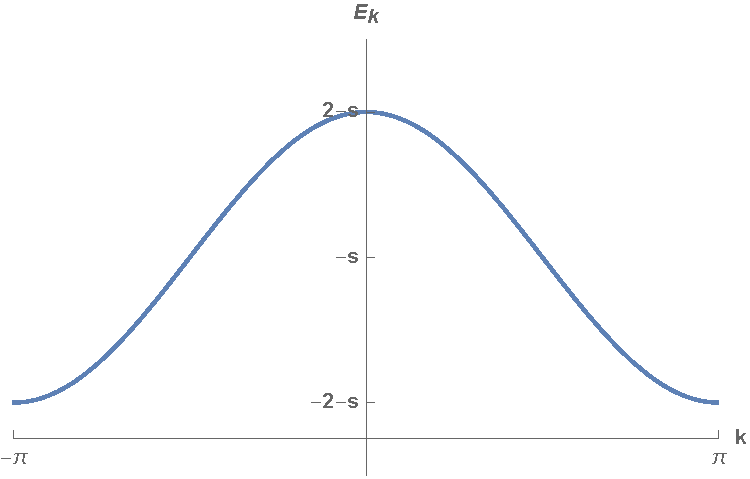
\includegraphics[width=1.0\textwidth]{HLTemplattBand}\\(a)
            \end{center}\end{minipage}
            \begin{minipage}[c]{0.3\textwidth}\begin{center}
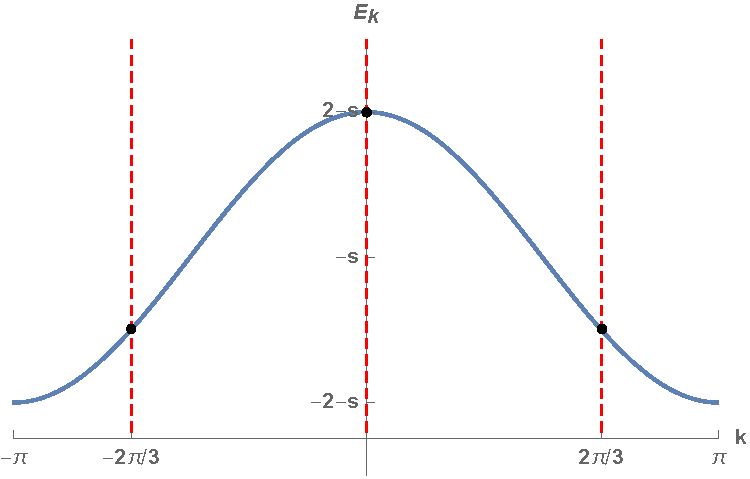
\includegraphics[width=1.0\textwidth]{HLTemplattBand3cycle}\\(b)
            \end{center}\end{minipage}
            \begin{minipage}[c]{0.3\textwidth}\begin{center}
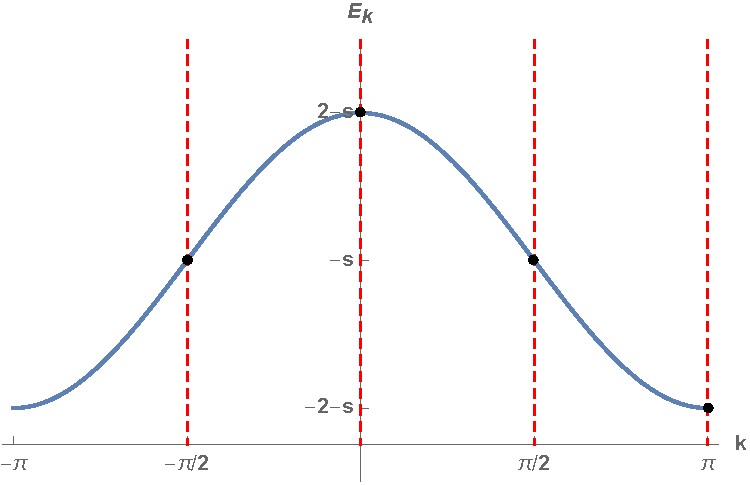
\includegraphics[width=1.0\textwidth]{HLTemplattBand4cycle}\\(c)
            \end{center}\end{minipage}
\end{center}
  \caption{\label{fig:LC21emplattBand}
(a) The eigenvalue $E_k$ of the \jacobianOrb\ on the infinite lattice as a function of the wave
vector $k$ in the first Brillouin zone. The \jacobianOrb\ has the reflection symmetry so the
eigenvalue is also invariant under the reflection $k\to -k$.
(b) For period 3 lattice states, the wave vectors of the eigenstates exist on the reciprocal lattice
spanned by $2\pi/3$. These lattice sites are labeled by the red dashed lines. There are only
3 period 3 eigenstates, with eigenvalues $-1-s$, $2-s$ and $-1-s$.
(c) For period 4 lattice states, the wave vectors of the eigenstates exist on the reciprocal lattice
spanned by $\pi/2$. These lattice sites are labeled by the red dashed lines. There are only
4 period 4 eigenstates, with eigenvalues $-s$, $2-s$, $-s$ and $-2-s$.
$k=\pi$ and $k=-\pi$ are different by a reciprocal lattice translation, so they are a same
wave vector and should be only counted once.
          }
\end{figure}
%%%%%%%%%%%%%%%%%%%%%%%%%%%%%%%%%%%%%%%%%%%%%%%

Explain \reffig{fig:LC21emplattBand}.

        \PC{2021-09-02} {
I think I prefer some version of the identity \refeq{TableOfISP13952},
\refeq{HillDetOrbJ},
no mention of Chebyshev polynomials. Not important, will revisit later.
    }


\subsection{Remarks}
\label{s:LC21HillForm}

Two remarks.
First, the reformulation of the \catlatt\ 3-term recurrence
% \refeq{CatMap2dHill}
as the `two-configuration' map \refeq{PV2config} is
a passage from the Lagrangian to the Hamiltonian formulation, also known
as `transfer matrix' formulation of lattice field
theories\rf{MonMun94,MunWal00} and Ising
models\rf{Onsager44,Kastening02}. We chose to prove it here using only
elementary linear algebra, not only because the Lagrangian
formalism\rf{BolTre10} is not needed for the problem at hand, but because
it actually obscures the generality of Hill's formula, which works
equally well for dissipative systems (see Bernoulli Hill's formula
\refeq{LC21PerViv}), systems with no Lagrangian formulation.
% use

Second,
for Hamiltonian evolution \refeq{catMap}, the $[2\!\times\!2]$
\jacobianM\ $\jMat^\cl{}$ (the monodromy matrix of a \po) describes
the growth of an initial state perturbation in $\cl{}$ steps. For the
corresponding Lagrangian system with action $\action$,
% (see \refsect{s:catLagrForm}),
the first variation of
the action $\delta\action=0$ yields the \templatt\ condition
\refeq{catTempLatt}, while the second variation, the
$[\cl{}\!\times\!\cl{}]$ {\jacobianOrb} \refeq{tempCatFix},
describes the stability of the \emph{entire} given \po. In this,
classical mechanics context, Bolotin and Treschev\rf{BolTre10} refer to
$\jMorb$ as the `Hessian operator', but, as it is clear from our
Bernoulli discussion of \refsect{s:JacobianOrb}, and applications to \KS\
and Navier-Stokes systems\rf{GuBuCv17}, this notion of global stability
of orbits is general, and applies to all dynamical systems, not only the
Hamiltonian ones.
